% File SDSS2020_SampleExtendedAbstract.tex
\documentclass[11pt]{article}
\usepackage{sdss2020} % Uses Times Roman font (either newtx or times package)
\usepackage{url}
\usepackage{latexsym}
\usepackage{amsmath, amsthm, amsfonts}
\usepackage{algorithm, algorithmic}
\usepackage{graphicx}
\usepackage{adjustbox}
\usepackage{setspace}
\setstretch{0.85}
\graphicspath{{images/}}

\title{Artificial Neural Networks and Deep Learning \\
Homework 2}

\author{
  Nicola Dean \\
  10674826 \\
  {\tt nicola.dean \\
  \tt @mail.polimi.it} \\\And
  Marco Fasanella \\
  10617541 \\
  {\tt marco.fasanella \\
  \tt @mail.polimi.it} \\\And
  Raffaello Fornasiere \\
    10790353 \\
    {\tt raffaello.fornasiere \\
    \tt @mail.polimi.it} \\\And
  Christian Spano \\
  10823764 \\
  {\tt christian.spano \\
  \tt @mail.polimi.it} \\}


\date{}

\begin{document}
\maketitle


\section{Introduction}


CHRISTIAN + MARCO
TIME SERIES MARCO
\begin{table}[h]
\begin{center}
\begin{tabular}{|l|rl|}
\hline \bf Type of Text & \bf Font Size & \bf Style \\ \hline
paper title & 15 pt & bold \\
author names & 12 pt & bold \\
author affiliation & 12 pt & \\
the word ``Abstract'' & 12 pt & bold \\
section titles & 12 pt & bold \\
document text & 10 pt  &\\
captions & 10 pt & \\
abstract text & 10 pt & \\
bibliography & 10 pt & \\
footnotes & 9 pt & \\
\hline
\end{tabular}
\end{center}
\caption{\label{fontsizes} Sizes and styles of fonts used.}
\end{table}

%What are time series??
%How to deal with them in short


%All our tries

\section{Preprocessing}
When it comes to TimeSeries classificaion/forecasting, preprocessing is a crucial step to grant optimal results.\
In this section will be described all the preprocessing techniques we tried or discarded.
\subsection{Normalization}
After visualizing the data, we noticed that samples has different scale factor based on targets.\
To avoid advantaging some of the classes we decided to normalize the dataset.
\subsubsection{Per Column}
As first approach, we normalized the dataset by \textbf{FULL columns}
\begin{itemize}
  \item \textbf{MinMax} Does not work properly; When applied, the validation accuracy dropped to 33%.
  \item \textbf{Mean / Std} This technique does not improve the accuracy on vanilla models.
\end{itemize}
\subsubsection{Per Sample}
The next method we tried, was to normalize each sample (TimeSerie) independently, to completly remove the different scales of the targets.
\begin{itemize}
  \item \textbf{MinMax} Improve performances but not enough, at least on vanilla models
  \item \textbf{Mean / Std} This was the \textbf{Game Changer} for us, it improves the performances on Vanilla models from 63\% to 67\%
\end{itemize}
\subsection{Augmentation}
In the Homework1 challenge, we noticed the importance of augmentation on this field and so we decided to give it a try also on time series.\
We tried both "by hand" and Library approach with the following results.
\subsubsection{Numpy}
Using the function \textit{np.random.normal} it is possible to generate random noise with a certain mean std and shape.\
To obtain augmented samples we copied the dataset multiple time, and then, for each time serie, we calculated it's standard deviation and applied the augmentation like follow:

\begin{figure}[h]
  \[ x = x + np.random.normal(0,std,x.shape) * w\]
  \caption{With x be a single time series, w be a weight of our choice}
\end{figure}

The result of augmantation was immediate and bring us a solid 68\% using the vanilla BiLstm
\subsubsection{TSUNG/Librery}
%Per raffaello, cambia il nome del titoletto come vuoi
 RAFFAELLO
\subsection{Seasonal + Trend preprocess}
Christian
\subsection{Expanding Window size}
\subsection{Adding New Features}
Christian
\section{Vanilla Models}
MARCO
\section{Net Concatenations}
\subsection{LSTM + CNN}
\subsection{CNN + LSTM}

\section{Heterogeneus Layers}
\subsection{LSTM + CNN}
\subsection{CNN + LSTM}

\subsection{CNN + DENSE}
\subsection{ALTRI DI RAFFAELLO}

\section{Our best Model}
Unexpectedly bla bla bla

\section{Conclusion}

\begin{figure}[h]
\centering
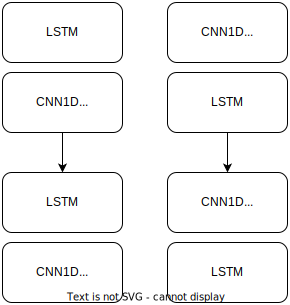
\includegraphics[width=6cm, height=4cm]{LSTMCNN}
\caption{LSTM-CNN and CNN-LSTM model schematics}
\end{figure}

\section{Adapt 2D models to 1D convolutions}
\subsection{InceptionNet}
\begin{figure}[h]
\centering
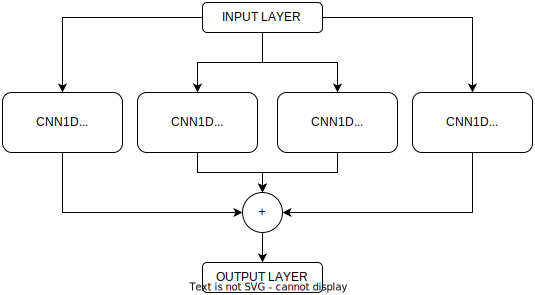
\includegraphics[width=6cm, height=4cm]{Inception}
\caption{CNN1D Inception Like Net}
\end{figure}

\subsection{Resnet}
\begin{figure}[h]
\centering
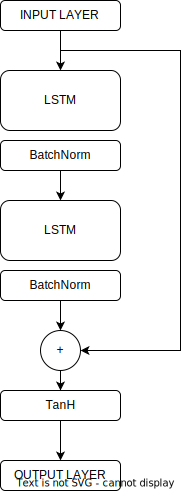
\includegraphics[width=4cm, height=8cm,angle =90]{resnet}
\caption{Resnet Like LSTM Net}
\end{figure}



\bibliographystyle{sdss2020} % Please do not change the bibliography style
\bibliography{SampleReferencesForExtendedAbstract}

\end{document}
